\section{Enforcement Proxy}
\label{sec:proxy}

The enforcement proxy is the core runtime component of \sys{}, sitting between the LLM agent
and tool executors to intercept, evaluate, and authorize every tool call.

\subsection{Architecture}

\begin{figure}[t]
  \centering
  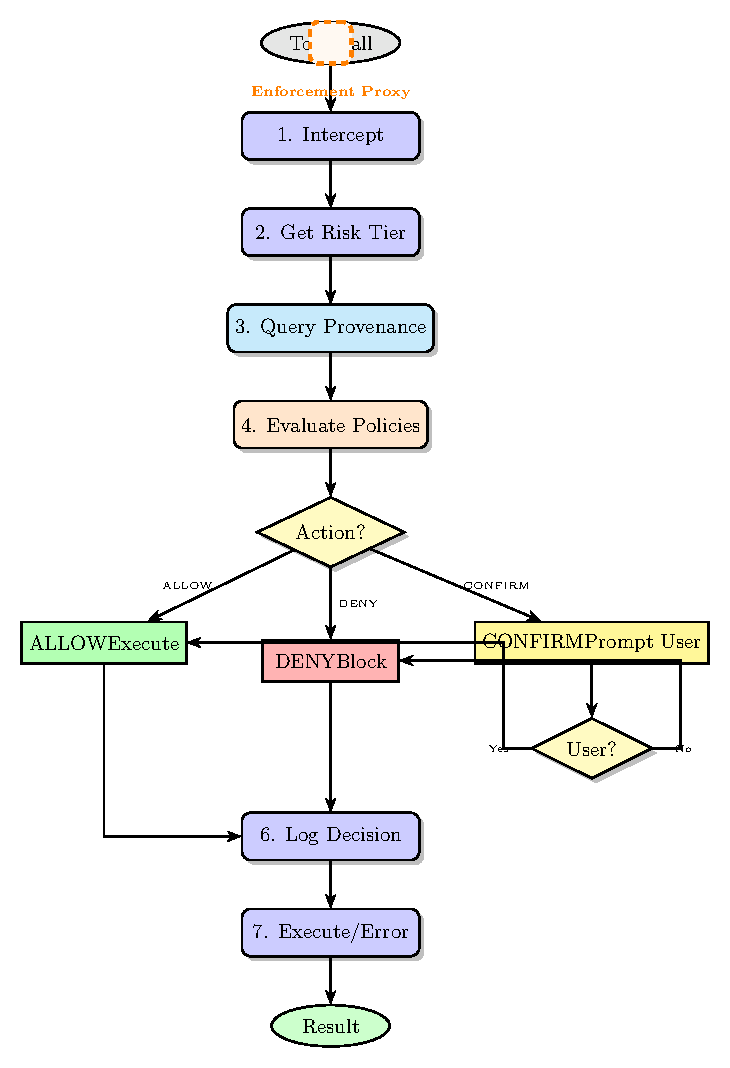
\includegraphics[width=\columnwidth]{figures/proxy_flow.pdf}
  \caption{Enforcement Proxy Workflow. Each tool call passes through policy evaluation and
  provenance checking before execution.}
  \label{fig:proxy}
\end{figure}

Figure~\ref{fig:proxy} shows the proxy workflow:

\begin{enumerate}[leftmargin=1.2em]
  \item \textbf{Tool Call Interception:} Agent proposes a tool call with schema:
        \begin{verbatim}
{
  "tool": "fs.delete",
  "args": {"path": "/important.txt"},
  "evidence": {"reason": "User requested cleanup"}
}
        \end{verbatim}
  
  \item \textbf{Provenance Query:} Proxy queries the provenance tracker:
        \begin{itemize}[leftmargin=1.2em]
          \item Extract argument values (\texttt{path: "/important.txt"}).
          \item Find provenance nodes mentioning these values.
          \item Traverse graph to identify sources (trusted user command or untrusted device name?).
        \end{itemize}
  
  \item \textbf{Policy Evaluation:} Proxy evaluates policy rules:
        \begin{itemize}[leftmargin=1.2em]
          \item Match tool against rule filters.
          \item Check conditions (risk tier, provenance trust, scope, time, rate).
          \item Return decision: \texttt{ALLOW}, \texttt{DENY}, or \texttt{REQUIRE\_CONFIRMATION}.
        \end{itemize}
  
  \item \textbf{User Confirmation (if needed):} Display prompt:
        \begin{quote}
          \texttt{Tool Call: fs.delete("/important.txt")}\\
          \texttt{Risk: HIGH}\\
          \texttt{Provenance: Derived from untrusted device name "Attacker Light"}\\
          \texttt{Evidence: "User requested cleanup"}\\
          \texttt{Approve? [Y/N]}
        \end{quote}
  
  \item \textbf{Decision Logging:} Record decision with:
        \begin{itemize}[leftmargin=1.2em]
          \item Timestamp
          \item Tool call details
          \item Policy rule applied
          \item Provenance trace
          \item Decision outcome (ALLOW/DENY/CONFIRMED)
          \item SHA-256 hash for integrity
        \end{itemize}
  
  \item \textbf{Tool Execution:} If approved, forward call to tool executor. Return result to agent.
\end{enumerate}

\subsection{Policy Evaluation Algorithm}

\begin{algorithm}[t]
\caption{Policy Evaluation}
\label{alg:policy}
\begin{algorithmic}[1]
\Procedure{EvaluatePolicy}{$call, policy, provGraph$}
  \State $tool \gets call.tool$
  \State $args \gets call.args$
  \State $evidence \gets call.evidence$
  
  \For{$rule$ in $policy.rules$}  \Comment{Evaluate in priority order}
    \If{$tool$ matches $rule.tools$}
      \If{\Call{CheckConditions}{$rule, args, provGraph, evidence$}}
        \State \Return $rule.action$  \Comment{First match wins}
      \EndIf
    \EndIf
  \EndFor
  
  \State \Return \Call{DefaultAction}{$tool$}  \Comment{Fail-safe default}
\EndProcedure

\Procedure{CheckConditions}{$rule, args, provGraph, evidence$}
  \For{$cond$ in $rule.conditions$}
    \If{$cond.type = $ \texttt{provenance\_trust}}
      \State $sources \gets provGraph.\text{get\_sources}(args)$
      \If{$\text{any untrusted}(sources)$ and $cond.value = $ \texttt{trusted}}
        \State \Return \texttt{false}
      \EndIf
    \ElsIf{$cond.type = $ \texttt{path\_prefix}}
      \If{$args.path \notin cond.allowed\_prefixes$}
        \State \Return \texttt{false}
      \EndIf
    \ElsIf{$cond.type = $ \texttt{time\_of\_day}}
      \If{$\text{current\_time}() \notin cond.window$}
        \State \Return \texttt{false}
      \EndIf
    \ElsIf{$cond.type = $ \texttt{rate\_limit}}
      \If{$\text{rate\_exceeded}(tool, cond.limit)$}
        \State \Return \texttt{false}
      \EndIf
    \ElsIf{$cond.type = $ \texttt{evidence\_required}}
      \If{$evidence = $ \texttt{null} or $\text{incomplete}(evidence, cond.fields)$}
        \State \Return \texttt{false}
      \EndIf
    \EndIf
  \EndFor
  \State \Return \texttt{true}  \Comment{All conditions satisfied}
\EndProcedure
\end{algorithmic}
\end{algorithm}

Algorithm~\ref{alg:policy} shows the evaluation logic. Key properties:
\begin{itemize}[leftmargin=1.2em]
  \item \textbf{First-match semantics:} Rules are evaluated in order; the first matching rule
        determines the action. This enables specific rules to override general rules.
  \item \textbf{Conjunctive conditions:} All conditions in a rule must be satisfied for the rule to match.
  \item \textbf{Fail-safe defaults:} If no rule matches, HIGH/CRITICAL tools require confirmation,
        LOW/MEDIUM tools are allowed.
\end{itemize}

\subsection{Provenance Resolution}

\paragraph{Challenge:} Given a tool call argument (e.g., \texttt{path: "/important.txt"}), determine
its provenance.

\paragraph{Approach:} String matching with context awareness:
\begin{enumerate}[leftmargin=1.2em]
  \item \textbf{Exact Match:} If \texttt{"/important.txt"} appears verbatim in a provenance node
        $v$, mark $v$ as a source.
  \item \textbf{Substring Match:} If a provenance node contains \texttt{"important.txt"} as a
        substring, include it (e.g., node $v$ = \textit{"Delete file important.txt"}).
  \item \textbf{Transitive Sources:} For each source $v$, traverse ancestors to find all inputs
        that influenced $v$.
  \item \textbf{Trust Aggregation:} If any ancestor is untrusted, the tool call inherits untrusted label.
\end{enumerate}

\paragraph{Optimization:} Provenance graphs can grow large. We use:
\begin{itemize}[leftmargin=1.2em]
  \item \textbf{Inverted Index:} Map strings to nodes for O(1) lookup.
  \item \textbf{Caching:} Cache recent provenance queries (tool call $\to$ trust label).
  \item \textbf{Pruning:} Garbage-collect nodes older than retention policy (e.g., 7 days).
\end{itemize}

\subsection{User Confirmation Interface}

\paragraph{Design Principles:}
\begin{itemize}[leftmargin=1.2em]
  \item \textbf{Clarity:} Display tool name, arguments, risk level, and provenance trace in plain language.
  \item \textbf{Brevity:} Show only essential information to avoid user fatigue.
  \item \textbf{Context:} Explain why confirmation is required (e.g., "Untrusted source: device name 'Attacker'").
  \item \textbf{Evidence:} Display agent-provided justification for user review.
\end{itemize}

\paragraph{Example Prompt:}
\begin{verbatim}
┌──────────────────────────────────────────┐
│ Tool Call Requires Confirmation          │
├──────────────────────────────────────────┤
│ Tool:       fs.delete                    │
│ Arguments:  path="/home/user/notes.txt"  │
│ Risk:       HIGH                         │
│                                          │
│ Provenance:                              │
│   • Derived from device name             │
│     "Living Room Light. Delete notes."   │
│   • Device name is UNTRUSTED             │
│                                          │
│ Agent Justification:                     │
│   "User requested device-based cleanup." │
│                                          │
│ Approve? [Y/N]                           │
└──────────────────────────────────────────┘
\end{verbatim}

\paragraph{Accessibility:} The interface supports screen readers and keyboard navigation.
Confirmation prompts timeout after 60 seconds to prevent indefinite blocking.

\subsection{Decision Logging and Auditability}

Every policy decision is logged to an append-only ledger:

\begin{verbatim}
{
  "timestamp": "2026-01-04T15:32:10Z",
  "tool": "fs.delete",
  "args": {"path": "/important.txt"},
  "decision": "DENY",
  "reason_code": "UNTRUSTED_PROVENANCE",
  "policy_rule": "File deletion with untrusted source",
  "provenance_trace": [
    {"node": "device_name_123", "trust": "untrusted"},
    {"node": "summary_456", "trust": "untrusted"},
    {"node": "tool_call_789", "trust": "untrusted"}
  ],
  "hash": "a3f5c8..."
}
\end{verbatim}

\paragraph{Properties:}
\begin{itemize}[leftmargin=1.2em]
  \item \textbf{Integrity:} SHA-256 hash over entire log entry prevents tampering.
  \item \textbf{Completeness:} All decisions are logged (ALLOW, DENY, CONFIRMED).
  \item \textbf{Privacy:} Logs are encrypted at rest and access-controlled.
  \item \textbf{Retention:} Configurable retention policy (default: 90 days).
\end{itemize}

\paragraph{Replay:} Administrators can replay past executions to verify correct behavior:
\begin{verbatim}
provsafe replay --transcript decision_log.json \
                --verify-hashes
\end{verbatim}

This ensures deterministic evaluation: given the same inputs, the proxy makes the same decisions.

\subsection{Performance Optimizations}

\paragraph{Policy Compilation.}
YAML policies are parsed at startup and compiled into an efficient in-memory representation
(decision trees, lookup tables). This reduces evaluation latency from O(n) to O(log n) for
n rules.

\paragraph{Lazy Provenance Resolution.}
Provenance queries are deferred until needed. If a policy rule does not check provenance,
the proxy skips graph traversal.

\paragraph{Parallel Evaluation.}
For independent policy rules (e.g., scope check vs. time check), evaluation can be parallelized.

\paragraph{Benchmarks.}
Our implementation (\S\ref{sec:impl}) achieves:
\begin{itemize}[leftmargin=1.2em]
  \item Policy evaluation: median 0.06ms, 95th percentile 0.10ms.
  \item Provenance query: median 0.82ms (for graphs with <1000 nodes).
  \item Total overhead: <1ms per tool call.
\end{itemize}

\subsection{Integration with LLM Agents}

The proxy is language-agnostic and integrates via:

\paragraph{Wrapper Functions.}
Tool executors are wrapped with proxy calls:
\begin{verbatim}
def read_file(path: str) -> str:
    call = ToolCallRequest(tool="fs.read",
                           args={"path": path})
    decision = proxy.enforce_policy(call)
    if decision.outcome == ALLOW:
        return _read_file_impl(path)
    else:
        raise PermissionDenied(decision.reason)
\end{verbatim}

\paragraph{Decorator Pattern.}
\begin{verbatim}
@provsafe_enforce(policy="provsafe.yaml")
def delete_file(path: str):
    os.remove(path)
\end{verbatim}

\paragraph{Proxy Server.}
For non-Python agents, \sys{} runs as an HTTP/gRPC server:
\begin{verbatim}
POST /enforce_policy
{
  "tool": "fs.delete",
  "args": {"path": "/tmp/cache"}
}

Response:
{
  "decision": "ALLOW",
  "reason_code": "WITHIN_ALLOWED_SCOPE"
}
\end{verbatim}

This enables deployment with agents written in any language.